%Triangles (C4ch37 et HM)
%-ok Inégalité triangulaire et droites remarquables
%-ok Déterminer l'existence d'un triangle à l'aide des longueurs de trois côtés
%-ok Hauteurs, médianes d'un triangle et applications
%-ok Médiatrices d'un triangle et cercle circonscrit à un triangle
%-ok Problèmes de construction divers

\chapter{Triangles}


\section{Rappels}
\id{Mathematic erklären an schon den 2 an 3 als Hausaufgab maachen loossen.}
\begin{center}
	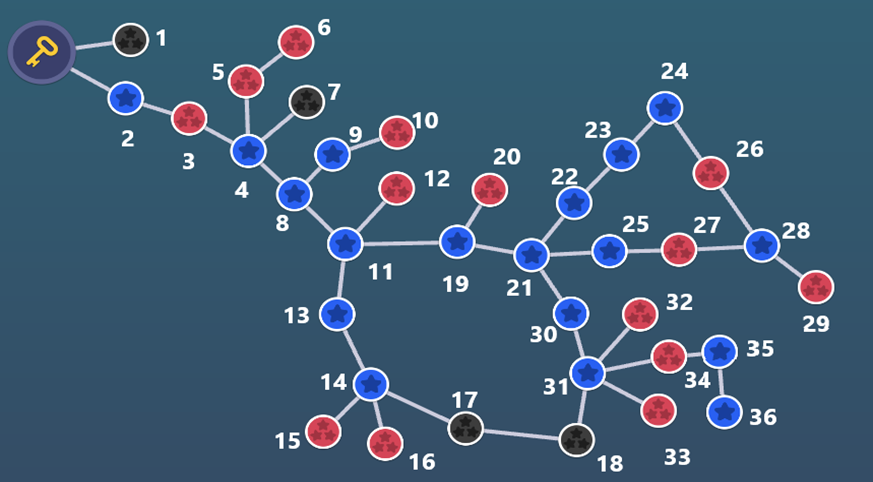
\includegraphics[width=9cm]{pictures/mathematic_angles_et_constructions.png}
\end{center}


\id{Tracer un triangle et une hauteur}

\defn{Une \emph{hauteur d'un triangle} est une droite qui passe par un sommet du triangle et qui est perpendiculaire au côté opposé à ce sommet.
}
\id{Tracer les autres hauteurs}

\rem{Les hauteurs d'un triangle se coupent en un point (sont concourantes).
Ce point est appelé l'\uline{orthocentre du triangle}.
}


%\arrow Ex. 33, 34 p.162 (T5) \datei{Bicher/T5/T5_p.162.jpg} \\
%\arrow Ex. 47 p.163 \datei{Bicher/T5/T5_p.163.jpg} \\
%\arrow Ex. 28, 31, 38 p.162 \\
%\arrow Ex. 45, 46 p.163



\section{La médiane}
\addexo{Pour chacun des triangles suivants, la droite $(AD)$ coupe les triangles en deux autres triangles.
Compare les surfaces des deux nouveaux triangles et explique la construction de la droite $(AD)$ à l'aide des sommets $A$, $B$ et $C$ seulement.
\begin{center}
\begin{tikzpicture}
	\draw[color=gro,dash pattern=on 1pt off 1pt, xstep=.5cm,ystep=.5cm] (-.2,-.2) grid (3.2,2.2);
	\draw (0,0)node[left]{$B$}
				--node[below](D){$D$} (3,0)node[right]{$C$}
				-- (1.5,2)node[above](A){$A$}
				--cycle;
	\draw[red] (A) --(D);
\end{tikzpicture}
\begin{tikzpicture}[scale=.7]
	\draw[color=gro,dash pattern=on 1pt off 1pt, xstep=1cm,ystep=1cm] (-.2,-2.2) grid (3.2,2.2);
	\draw (3,2)node[right]{$B$}
				--node[right](D){$D$} (3,-2)node[right]{$C$}
				-- (0,0)node[left](A){$A$}
				--cycle;
	\draw[red] (A) --(D);
\end{tikzpicture}
\begin{tikzpicture}[scale=.7]
	\draw[color=gro,dash pattern=on 1pt off 1pt, xstep=.5cm,ystep=.5cm] (-.2,.2) grid (2.2,-4.2);
	\draw (0,-4)node[left]{$B$}
				--node[below right](D){$D$} (2,0)node[right]{$C$}
				-- (0,0)node[above](A){$A$}
				--cycle;
	\draw[red] (0,0) --(1,-2);
	\draw[blue!20] (1,0) --(1,-2) --(0,-2);
\end{tikzpicture}
\begin{tikzpicture}[scale=.8]
	\draw[color=gro,dash pattern=on 1pt off 1pt, xstep=.5cm,ystep=.5cm] (-.2,-.2) grid (4.2,3.2);
	\draw (0,0)node[left]{$B$}
				--node[below](D){$D$} (4,1)node[right]{$C$}
				-- (1,3)node[above](A){$A$}
				--cycle;
	\draw[red] (1,3) --(2,.5);
\end{tikzpicture}
\end{center}
%\begin{center}
%\definecolor{qqzzqq}{rgb}{0.,0.6,0.}
%\definecolor{ttttff}{rgb}{0.2,0.2,1.}
%\definecolor{ffqqqq}{rgb}{1.,0.,0.}
%\definecolor{qqqqff}{rgb}{0.,0.,1.}
%\definecolor{cqcqcq}{rgb}{0.7529411764705882,0.7529411764705882,0.7529411764705882}
%\begin{tikzpicture}[scale=.6,line cap=round,line join=round,>=triangle 45,x=1.0cm,y=1.0cm]
%	\draw [color=cqcqcq,dash pattern=on 1pt off 1pt, xstep=1.0cm,ystep=1.0cm] (0.4204876451923835,0.5616892144800908) grid (5.579050674208538,5.660730362392205);
%	\clip(0.4204876451923835,0) rectangle (5.579050674208538,5.660730362392205);
%	\fill[color=ttttff,fill=ttttff,fill opacity=0.1] (5.,1.) -- (3.,5.) -- (3.,1.) -- cycle;
%	\fill[color=qqzzqq,fill=qqzzqq,fill opacity=0.1] (3.,1.) -- (3.,5.) -- (1.,1.) -- cycle;
%	\draw [color=ffqqqq] (3.,0.5616892144800908) -- (3.,5.660730362392205);
%	\draw [color=ttttff] (5.,1.)-- (3.,5.);
%	\draw [color=ttttff] (3.,5.)-- (3.,1.);
%	\draw [color=ttttff] (3.,1.)-- (5.,1.);
%	\draw [color=qqzzqq] (3.,1.)-- (3.,5.);
%	\draw [color=qqzzqq] (3.,5.)-- (1.,1.);
%	\draw [color=qqzzqq] (1.,1.)-- (3.,1.);
%	\draw [fill=qqqqff] (3.,5.) circle (1.5pt);
%	\draw[color=qqqqff] (3.1386535489432035,5.283758448733333) node {$A$};
%	\draw [fill=qqqqff] (1.,1.) circle (1.5pt);
%	\draw[color=qqqqff] (0.7974595588512564,1.256111160693803) node {$B$};
%	\draw [fill=qqqqff] (5.,1.) circle (1.5pt);
%	\draw[color=qqqqff] (5.142556879445633,1.2759517877284803) node {$C$};
%	\draw [fill=ffqqqq] (3.,1.) circle (1.5pt);
%	\draw[color=ffqqqq] (2.7,1) node[below] {$D$};
%	\draw[color=ffqqqq] (3.2180160570819134,8.835230687940603) node {$d$};
%\end{tikzpicture}
%\hspace{.25cm}
%\definecolor{qqzzqq}{rgb}{0.,0.6,0.}
%\definecolor{ttttff}{rgb}{0.2,0.2,1.}
%\definecolor{ffqqqq}{rgb}{1.,0.,0.}
%\definecolor{qqqqff}{rgb}{0.,0.,1.}
%\definecolor{cqcqcq}{rgb}{0.7529411764705882,0.7529411764705882,0.7529411764705882}
%\begin{tikzpicture}[scale=.6,line cap=round,line join=round,>=triangle 45,x=1.0cm,y=1.0cm]
%	\draw [color=cqcqcq,dash pattern=on 1pt off 1pt, xstep=1.0cm,ystep=1.0cm] (0.5593720344351262,0.5815298415147683) grid (5.777456944555313,3.498102015612359);
%	\clip(0.5593720344351262,0.5815298415147683) rectangle (5.777456944555313,3.498102015612359);
%	\fill[color=ttttff,fill=ttttff,fill opacity=0.1] (5.,3.) -- (1.,2.) -- (5.,2.) -- cycle;
%	\fill[color=qqzzqq,fill=qqzzqq,fill opacity=0.1] (5.,2.) -- (1.,2.) -- (5.,1.) -- cycle;
%	\draw [color=ffqqqq,domain=0.5593720344351262:5.777456944555313] plot(\x,{(--8.-0.*\x)/4.});
%	\draw [color=ttttff] (5.,3.)-- (1.,2.);
%	\draw [color=ttttff] (1.,2.)-- (5.,2.);
%	\draw [color=ttttff] (5.,2.)-- (5.,3.);
%	\draw [color=qqzzqq] (5.,2.)-- (1.,2.);
%	\draw [color=qqzzqq] (1.,2.)-- (5.,1.);
%	\draw [color=qqzzqq] (5.,1.)-- (5.,2.);
%	\draw [fill=qqqqff] (1.,2.) circle (1.5pt);
%	\draw[color=qqqqff] (0.9561845751286765,2.3076643935317094) node {$A$};
%	\draw [fill=qqqqff] (5.,1.) circle (1.5pt);
%	\draw[color=qqqqff] (5.182238133514987,1.2362705336591253) node {$B$};
%	\draw [fill=qqqqff] (5.,3.) circle (1.5pt);
%	\draw[color=qqqqff] (5.142556879445633,3.2798551182309064) node {$C$};
%	\draw [fill=ffqqqq] (5.,2.) circle (1.5pt);
%	\draw[color=ffqqqq] (5.221919387584343,1.83148934469945) node {$D$};
%	\draw[color=ffqqqq] (-5.035684789343934,2.327505020566387) node {$d$};
%\end{tikzpicture}
%\end{center}
%%
%\begin{center}
%\definecolor{qqzzqq}{rgb}{0.,0.6,0.}
%\definecolor{ttttff}{rgb}{0.2,0.2,1.}
%\definecolor{ffqqqq}{rgb}{1.,0.,0.}
%\definecolor{qqqqff}{rgb}{0.,0.,1.}
%\definecolor{cqcqcq}{rgb}{0.7529411764705882,0.7529411764705882,0.7529411764705882}
%\begin{tikzpicture}[scale=.6,line cap=round,line join=round,>=triangle 45,x=1.0cm,y=1.0cm]
%	\draw [color=cqcqcq,dash pattern=on 1pt off 1pt, xstep=1.0cm,ystep=1.0cm] (1.392678369891582,0.5220079604107358) grid (6.551241398907736,3.6568270318897786);
%	\clip(1.392678369891582,0.5220079604107358) rectangle (6.551241398907736,3.6568270318897786);
%	\fill[color=ttttff,fill=ttttff,fill opacity=0.1] (6.,1.) -- (3.,3.) -- (4.,1.) -- cycle;
%	\fill[color=qqzzqq,fill=qqzzqq,fill opacity=0.1] (4.,1.) -- (3.,3.) -- (2.,1.) -- cycle;
%	\draw [color=ffqqqq,domain=1.392678369891582:6.551241398907736] plot(\x,{(--9.-2.*\x)/1.});
%	\draw [color=ttttff] (6.,1.)-- (3.,3.);
%	\draw [color=ttttff] (3.,3.)-- (4.,1.);
%	\draw [color=ttttff] (4.,1.)-- (6.,1.);
%	\draw [color=qqzzqq] (4.,1.)-- (3.,3.);
%	\draw [color=qqzzqq] (3.,3.)-- (2.,1.);
%	\draw [color=qqzzqq] (2.,1.)-- (4.,1.);
%	\draw [fill=qqqqff] (3.,3.) circle (1.5pt);
%	\draw[color=qqqqff] (3.1386535489432035,3.2798551182309064) node {$A$};
%	\draw [fill=qqqqff] (2.,1.) circle (1.5pt);
%	\draw[color=qqqqff] (1.8093315376198098,1.256111160693803) node {$B$};
%	\draw [fill=qqqqff] (6.,1.) circle (1.5pt);
%	\draw[color=qqqqff] (6.134588231179508,1.2759517877284803) node {$C$};
%	\draw [fill=ffqqqq] (4.,1.) circle (1.5pt);
%	\draw[color=ffqqqq] (3.733872359983529,0.7997767388962207) node {$D$};
%	\draw[color=ffqqqq] (0.32128451001899594,8.835230687940603) node {$d$};
%\end{tikzpicture}
%\hspace{.25cm}
%\definecolor{qqzzqq}{rgb}{0.,0.6,0.}
%\definecolor{ttttff}{rgb}{0.2,0.2,1.}
%\definecolor{ffqqqq}{rgb}{1.,0.,0.}
%\definecolor{qqqqff}{rgb}{0.,0.,1.}
%\definecolor{cqcqcq}{rgb}{0.7529411764705882,0.7529411764705882,0.7529411764705882}
%\begin{tikzpicture}[scale=.6,line cap=round,line join=round,>=triangle 45,x=1.0cm,y=1.0cm]
%	\draw [color=cqcqcq,dash pattern=on 1pt off 1pt, xstep=1.0cm,ystep=1.0cm] (1.352997115822227,0.28392043599460604) grid (6.590922652977091,3.676667658924456);
%	\clip(1.352997115822227,0.28392043599460604) rectangle (6.590922652977091,3.676667658924456);
%	\fill[color=ttttff,fill=ttttff,fill opacity=0.1] (6.,3.) -- (2.,3.) -- (4.,2.) -- cycle;
%	\fill[color=qqzzqq,fill=qqzzqq,fill opacity=0.1] (4.,2.) -- (2.,3.) -- (2.,1.) -- cycle;
%	\draw [color=ffqqqq,domain=1.352997115822227:6.590922652977091] plot(\x,{(--8.-1.*\x)/2.});
%	\draw [color=ttttff] (6.,3.)-- (2.,3.);
%	\draw [color=ttttff] (2.,3.)-- (4.,2.);
%	\draw [color=ttttff] (4.,2.)-- (6.,3.);
%	\draw [color=qqzzqq] (4.,2.)-- (2.,3.);
%	\draw [color=qqzzqq] (2.,3.)-- (2.,1.);
%	\draw [color=qqzzqq] (2.,1.)-- (4.,2.);
%	\draw [fill=qqqqff] (2.,3.) circle (1.5pt);
%	\draw[color=qqqqff] (1.9680565538972299,3.3195363723002616) node {$A$};
%	\draw [fill=qqqqff] (2.,1.) circle (1.5pt);
%	\draw[color=qqqqff] (1.6307658943077121,0.978342382208318) node {$B$};
%	\draw [fill=qqqqff] (6.,3.) circle (1.5pt);
%	\draw[color=qqqqff] (6.134588231179508,3.2798551182309064) node {$C$};
%	\draw [fill=ffqqqq] (4.,2.) circle (1.5pt);
%	\draw[color=ffqqqq] (4.2100474088157895,1.83148934469945) node {$D$};
%	\draw[color=ffqqqq] (-5.035684789343934,6.335311681571239) node {$d$};
%\end{tikzpicture}
%\end{center}
}{-}

\defn{Une \emph{médiane d'un triangle} passe par un sommet et par le milieu du côté opposé à ce sommet.
}

\prop{Une médiane partage le triangle en deux surfaces de même aire.
}

\id{Tracer un triangle avec ces 3 médianes.}


\prop{Le point d'intersection des médianes d'un triangle est le centre de gravité de ce triangle. \\
C'est le \og point d'équilibre\fg{} de ce triangle.
}

\addexo{Construire le triangle $\Delta ABC$ tel que 
$$ \widehat{A}=70\degres\; AB=5\, cm\; BC=6\, cm. $$
Puis, construire la médiane issue de $B$.
}{-}

\addexo{Construire un triangle rectangle ainsi que ses trois médianes.
}{-}





\section{L'inégalité triangulaire}
Mathematic:
\begin{enumerate}[label=$\rightarrow$]
	\item 2, 3: vocabulaire,
	\item 28, 29 module angles et constructions,
	\item 22,24,24 fir constructioun CCC, CAC, ACA.
\end{enumerate}
	


%%%% Aal Versioun firum avancé/base
%Introduction: Quel chemin est le plus vite? Le chemin direct ou la déviation?
%
%\prop[Inégalité triangulaire]{Soient $A, B$ et $C$ trois points. Alors
%$$ AC \leq AB+BC. $$
%}
%
%\defn{Un triangle $ABC$ est \emph{isocèle en $A$} ssi ${\green A}B = {\green A}C$.
%\definecolor{zzttqq}{rgb}{0.6,0.2,0}
%\definecolor{qqqqff}{rgb}{0,0,1}
%\definecolor{cqcqcq}{rgb}{0.75,0.75,0.75}
%\begin{center}
%\begin{tikzpicture}[line cap=round,line join=round,>=triangle 45,x=1.0cm,y=1.0cm]
%	\clip(-1.48,0.78) rectangle (2.58,3.5);
%	\fill[color=zzttqq,fill=zzttqq,fill opacity=0.1] (-1,2) -- (2,3) -- (2,1) -- cycle;
%	\draw [color=zzttqq] (-1,2)-- (2,3);
%	\draw [color=zzttqq] (0.44,2.57) -- (0.5,2.4);
%	\draw [color=zzttqq] (0.5,2.6) -- (0.56,2.43);
%	\draw [color=zzttqq] (2,3)-- (2,1);
%	\draw [color=zzttqq] (2,1)-- (-1,2);
%	\draw [color=zzttqq] (0.5,1.4) -- (0.56,1.57);
%	\draw [color=zzttqq] (0.44,1.43) -- (0.5,1.6);
%	\fill [color=qqqqff] (-1,2) circle (1.5pt);
%	\draw[color=qqqqff] (-1.22,1.86) node {$A$};
%	\fill [color=qqqqff] (2,3) circle (1.5pt);
%	\draw[color=qqqqff] (2.16,3.28) node {$B$};
%	\fill [color=qqqqff] (2,1) circle (1.5pt);
%	\draw[color=qqqqff] (2.3,1.0) node {$C$};
%\end{tikzpicture}
%\end{center}
%}
%

%\arrow Ex. 19, 21, 23 p.161 (T5) \\
%\arrow Ex. 57 p.164 \datei{Bicher/T5/T5_p.164.jpg} \\
%\arrow Ex. 64, 67, 68, 69 p.165 \datei{Bicher/T5/T5_p.165.jpg} \\
%\arrow Ex. 70, 74 p.166 \datei{Bicher/T5/T5_p.166.jpg} \\



\section{La médiatrice et la bissectrice}
Mathematic: items 13-18 module angles et constructions.

\id{Wann si déi éischt Stonn am Mathematic gemaacht hunn, mindestens items 13 an 14, dann an der nächser Stonn folgende Résumé opschreiwen.
}

\ret{La \textbf{médiatrice d'un segment}:
\begin{enumerate}[label=$\rightarrow$]
	\item passe perpendiculairement par le milieu de ce segment.
	\item est l'ensemble des les points qui sont équidistants des extrémités du segment.
\end{enumerate}
La \textbf{bissectrice d'un angle}:
\begin{enumerate}[label=$\rightarrow$]
	\item partage cet angle en deux angles de même amplitude.
	\item est l'ensemble des points qui sont équidistants des côtés de cet angle.
\end{enumerate}
}

%\defn{La \textbf{médiatrice d'un segment} passe perpendiculairement par le milieu de ce segment.}
%
%\id{Dreieck mat de médiatrices zeechnen.}
%
%\prop{La médiatrice est l'ensemble de tous les points qui sont à égale distance des extrémités du segment.
%}

\addexo{Construire un triangle quelconque $ABC$.
\begin{enumerate}
	\item Où sont situés les points qui sont équidistants des sommets $A$ et $B$?
	\item Construire l'ensemble de tous ces points.
	\item Où sont situés les points qui sont équidistants des sommets $B$ et $C$?
	\item Construire l'ensemble de tous ces points.
	\item Que peut-on dire du (des) point(s) d'intersection des deux ensembles ci-dessus par rapport aux trois sommets du triangle $ABC$?
\end{enumerate}
}{Conclusion: définition du centre du cercle circonscrit.
}

\defn{Le point d'intersection des médiatrices de deux (et donc aussi de trois) côtés d'un triangle est équidistant des trois sommets de ce triangle et appelé \textbf{centre du cercle circonscrit} à ce triangle.
}

%\addexo{Construire le triangle $\Delta MNP$ tel que 
%$$ \widehat{P}=130\degres\; MN=4\, cm\; MP=7\, cm. $$
%Puis, construire le centre du cercle circonscrit au $\Delta MNP$.
%}{-}
%
%\addexo{Construire un triangle rectangle ainsi que son centre du cercle circonscrit.
%}{-}



















%%% -------------------------------- EXERCICEN PRINTEN

\clearpage
\begin{exercices}
\foreach \x/\y in \exos
{\exo \x
% \ifnum\value{exo}=13 \columnbreak \fi
 }
\end{exercices}